In the prototypes TRITIUM-IFIC-0 and TRITIUM-IFIC-1, the fibers were directly coupled to the photosensor, so detected photons were only those guided along the fibers. However, in TRITIUM-Aveiro and TRITIUM-IFIC-2, two PMMA windows are used which allows the transmission to the photosensors of photons propagated through the water. To quantify the importance of this contribution, the TRITIUM-Aveiro prototype was simulated. The distribution of the number of photons that reach the PMMA per tritium event is shown in Figure \ref{fig:PMMAEffect}. Fiber-guided photons are shown in a red distribution, while those traveling in the water medium are plotted in the blue histogram. It can be seen that the tritium signal obtained from the water guided photons is as important as that obtained from the fibers. Therefore, PMMA windows improve tritium detection efficiency by an almost 2 factor.

\begin{figure}[hbtp]
\centering
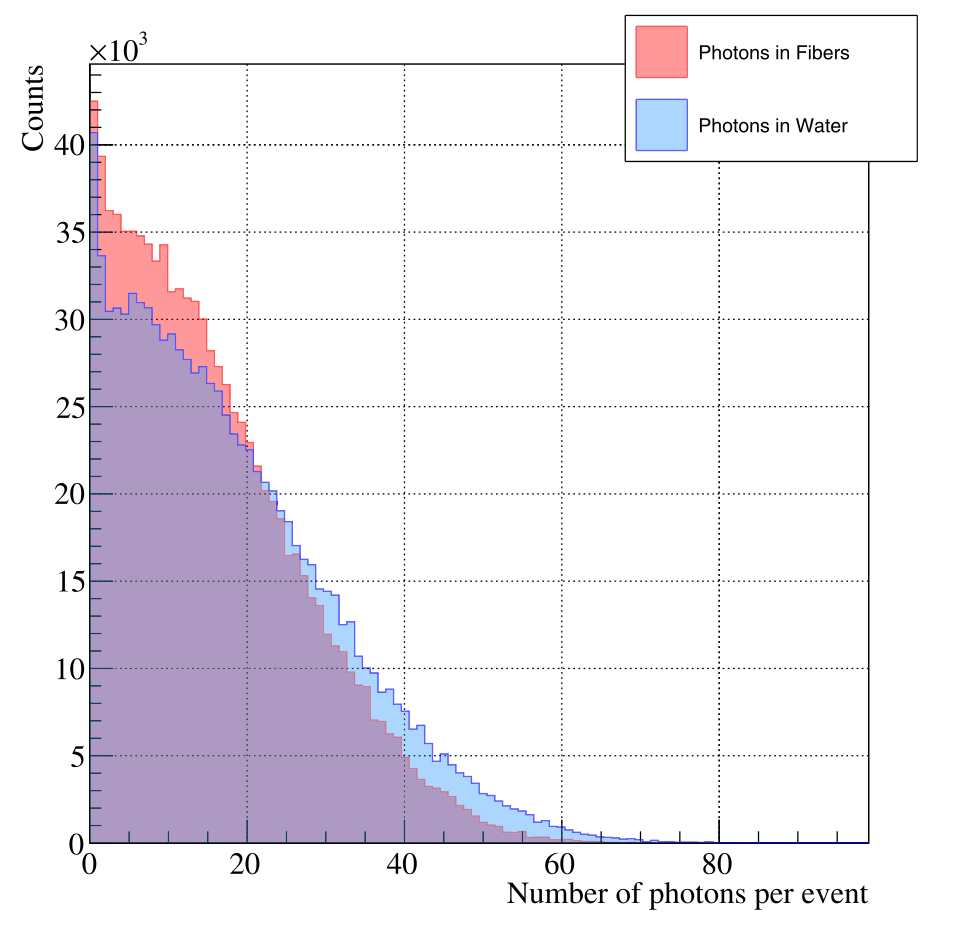
\includegraphics[scale=0.3]{6Simulations/61TRITIUMDesign/615PMMA/PhotonsDetectedWaterFiber.png}
\caption{Distribution of photons reaching the PMMA windows. The red histogram corresponds to the photons guided by fibers and the blue histogram to photons traveling in water \cite{SimulationPaperCarlos}.\label{fig:PMMAEffect}}
\end{figure}

